\chapter{Harmonic magnetic field in 2D - Induction heating of a graphite crucible}

\modinfo{Directory}{InductionHeatingGUI}
\modinfo{Solvers}{\Idx{MagnetoDynamics2DHarmonic}}
\modinfo{Tools}{\Idx{Gmsh}, \Idx{ElmerGUI}}
\modinfo{Dimensions}{2D, Axi-Symmetric}
\modinfo{Author}{Peter R{\aa}back}


\subsection*{Case definition}

At high temperatures the most practical 
method to heat up the crucible 
is by electromagnetic induction. 
The induction coil generates an alternating 
current that flows through the crucible. 
The Ohmic resistance encountered by this current dissipates 
energy, thereby directly
heating the crucible via internal heat generation.

The tutorial case is a simple axi-symmetric crucible that could be
used, for example, to grow silicon carbide (SiC) with physical vapour deposition.
The crucible 
is made of dense graphite and isolated by 
porous graphite. At the bottom of the crucible there is
some SiC powder. The physical properties of the 
material are given in Table~\ref{tab:ind_heat_a}. The dimensions of the
induction heating crucible are given in Table~\ref{tab:ind_heat_b}.

We neglect the helicity of the coil and assume an  
average current density that may be computed easily when the 
area of the coil is known, $j_0=n I / A$, where $A$ is the coil area.
Here we assume a current density of 1.0e6~A/m$^2$. 
The frequency of induction heating $f$ is assumed to be 50~kHz.

The permeability of vacuum is $4\pi 10^{-7}$
if the other variables are in SI-units. Relative permeability is assumed to be one in all materials. 

\begin{table}
\caption{Material parameters of the crucible}
\label{tab:ind_heat_a}
\begin{center}
\begin{tabular}{llll} \hline
material & $\varepsilon$  & $\kappa$ [W/mk] & $\sigma$ (1/$\Omega$m) \\ \hline 
graphite  &      0.7   &          10.0  &          2.0E4 \\
insulation &      0.9   &          1.0   &          2.0E3  \\
powder    &      0.5   &          25.0  &          1.0E4 \\ \hline
\end{tabular}
\end{center}
\end{table}

\begin{table}
\caption{Dimensions of the crucible}
\label{tab:ind_heat_b}
\begin{center}
\begin{tabular}{lllll} \hline
body part &  $r_{inner}$ & $r_{outer}$ & $h_{inner}$ & $h_{outer}$ \\ \hline
graphite  &  2.0   &  2.5 & 6.0 & 8.0 \\
insulation &  2.5   &  4.0 & 8.0 & 12.0 \\
coil      &  5.0   & 5.5  &     & 8.0  \\ \hline
\end{tabular}
\end{center}
\end{table}

\subsection*{Solution procedure}

The definitions for the relevant equation are not loaded into ElmerGUI by default. Hence, 
one needs to load these before starting the simulations.
\ttbegin
File 
  Definitions
    Append -> magnetodynamics2d.xml
\ttend
The additional definitions should reside in the directory \texttt{edf-extra} within the distribution.
Moving the desired \texttt{xml} files to the \texttt{edf}-directory enables automatic loading of the 
definitions at start-up. By inspecting the definitions in the \texttt{Elmer Definitions File editor} one
may inspect that the new definitions were really appended. 

The mesh is already defined, load it from the \texttt{samples} directory were it resides.
\ttbegin
File 
  Open -> crucible.msh
\ttend
The ElmerGrid plug-in of ElmerGUI will read the mesh and convert it to a format understood by Elmer. 

\begin{figure}[h]
\centering
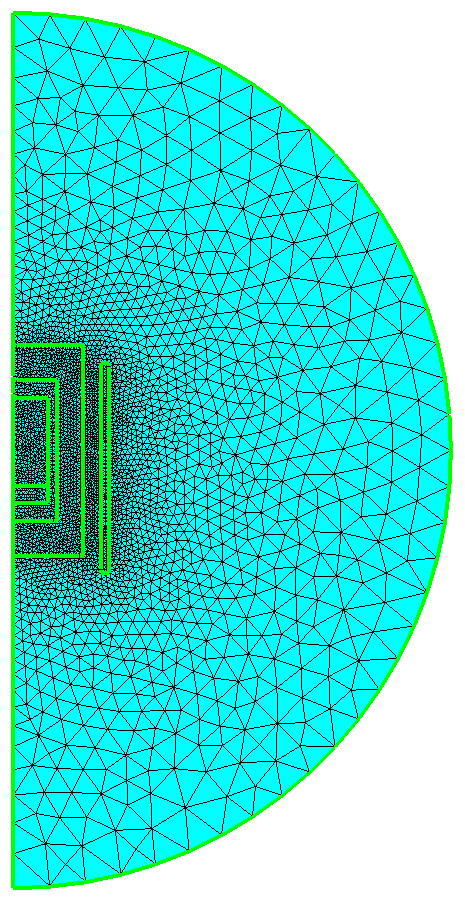
\includegraphics[width=60mm]{crucible_mesh}
\caption{The mesh for the horseshoe and surrounding air as see in ElmerGUI}\label{fg:crucible_mesh}
\end{figure}  


After we have the mesh we start to go through the Model menu from the top to bottom. 
In the Setup we choose things related to the whole simulation such as file names, 
time stepping, constants etc.
Currently the permeability of vacuum is not given
in the ElmerGUI. To set other than the default value for it, the free text box can be used. 
The steady-state simulation is carried out in rotationally symmetric 2-dimensional 
coordinates which must be changed.

\ttbegin
Model
  Setup  
    Coordinate system -> Axi symmetric
\ttend
 
In the equation section we choose the relevant equations and parameters related to their solution. 
In this case we'll have the MgDyn2DHarmonic solver, as well as the postprocessing solver MgDyn2DPost.

When defining Equations and Materials it is possible to assign to the bodies immediately, or to use mouse
selection to assign them later. In this case the equations need to be solved in all the bodies and 
hence clicking all from 1 to 6 here is most convenient. We give a higher priority to the actual solver
so that the vector potential will be computed before the derived fields. 
In this case solver specific options should be OK but they could also be changed in this context.
\ttbegin
Model
  Equation
	Solver -> MgDyn2DHarmonic
      Active = on
      Priority = 1
      Angular Frequency = 50.0e3
      Apply to Bodies = 1 2 3 4 5 6
    Solver -> MgDyn2DPost
      Active = on
      Edit Solver Settings
        Solver Specific Options
          Target Variable Complex = on
          Calculate Joule Heating = on
    Name = Induction
    Add 
    OK
\ttend        
The Material section includes all the material parameters. In this case we basically have two 
different materials but the different magnetization must also be given as a material property.
Hence we actually need to define four materials. The thermal properties are not needed at this stage as 
we are only solving for the induction. The internal losses of the coil are omitted and it is treated as an
pure current source with material properties of air.  
\ttbegin
Model
  Material
    Name = Air
    MgDyn2dHarmonic
      Relative Permeability = 1.0
      Electric Conductivity = 0.0
    Add
    New
	
    Name = Graphite
    MgDyn2dHarmonic
      Relative Permeability = 1.0
      Electric Conductivity = 2.0e4
    Add
    New

    Name = Insulation
    MgDyn2dHarmonic
      Relative Permeability = 1.0
      Electric Conductivity = 2.0e3
    Add
    New

    Name = Powder
    MgDyn2dHarmonic
      Relative Permeability = 1.0
      Electric Conductivity = 1.0e4
    Add
    New
\ttend

We may now assign the material properties by selecting with the mouse.
This spares us of the 
need to know the indexes of each body.
\ttbegin
Model
  Set body properties
    Choose external air -> set Material to Air
    Choose coil -> set Material to Air
    Choose insulation (outermost body) -> set Material to Insulation
    Choose graphite (actual crucible) -> set Material to Graphite
    Choose powder at the bottom of crucible -> set Material to Powder
    Choose internal air above the powder-> set Material to Air
\ttend

We need to provide a current source in order for the equation to have a nontrivial solution.
\ttbegin
Model
  BodyForce
    Name = CurrentSource
    MgDyn2DHarmonic
      Current Density = 2.5e5
    Add
    OK
\ttend   
This must be also joinded with the coil
\ttbegin
Model
  Set body properties
    Choose coil -> set Body force to CurrentSource
\ttend


We have just one boundary condition i.e. the outer boundary for which we use the farfield condition.
\ttbegin
Model
  BoundaryCondition
    Name = Farfield
    MgDyn2DHarmonic
      Infinity BC = True
    Add
    OK
\ttend   

The conditions may also be assigned to boundaries in the Boundary condition menu, or 
by clicking with the mouse. Here we use the latter approach as that spares us of the 
need to know the indexes of each boundary.
\ttbegin
Model
  Set boundary properties
    Choose the 2 pieces of the exterior -> set boundary condition Farfield
\ttend

For the execution 
ElmerSolver needs the mesh files and the command file. We have now basically defined
all the information for ElmerGUI to write the command file. After writing it we may also visually 
inspect the command file.
\ttbegin
Sif 
  Generate
  Edit -> look how your command file came out  
\ttend

Before we can execute the solver we should save the files in a directory. The project includes
all the files needed to restart the case.
\ttbegin
File 
  Save Project
\ttend

After we have successfully saved the files we may start the solver
\ttbegin
Run
  Start solver
\ttend
A convergence view automatically pops up showing relative changes of each iteration.
The equation is fully linear and hence only two iterations are needed -- the second 
one just ensures that convergence of the non-linear level was really obtained. 
The norm of the solution should be 0.3679.



When the solution has finished we may start the postprocessor to view some results.
\ttbegin
Run
  Start ParaView
\ttend


With the given computational mesh the problem is solved in 
a few seconds. With the 6\,542 linear triangles the heating
efficieny is estimated to be 18.9~W. The corresponding results are shown
in Fig.~\ref{fig:ind_heat1}.

It can be noted that would the estimated heating efficiency be different from the known one
the user may give the postpressing solver the \texttt{Desired Heating Power} in order to scale 
the potential of the solution. The solution, on the other hand, may be used as a source term 
in heat equation, for example. 

\begin{figure}
\begin{center}
  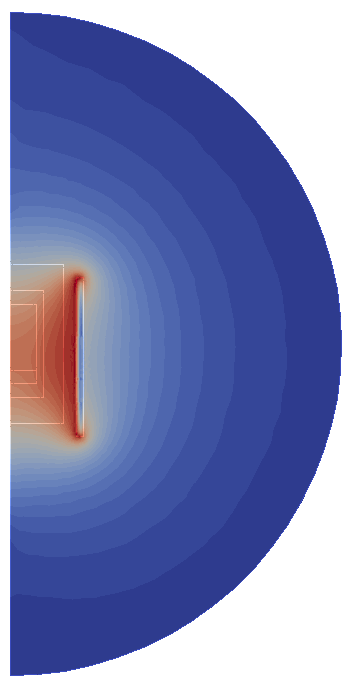
\includegraphics[height=60mm]{Induction_B_re}
  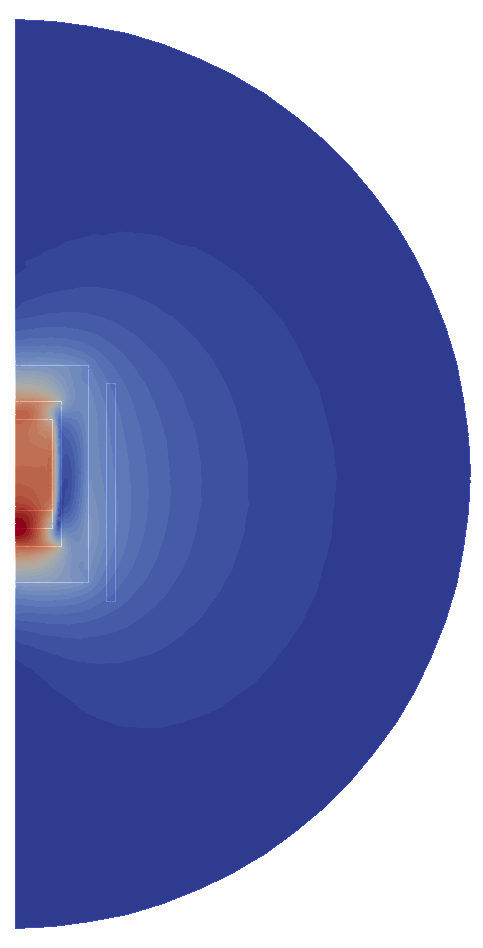
\includegraphics[height=60mm]{Induction_B_im}
  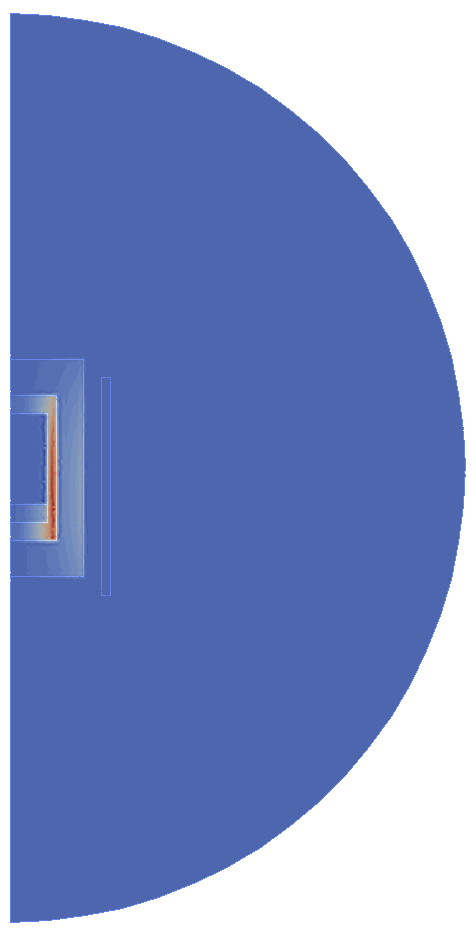
\includegraphics[height=60mm]{Induction_Joule_heating}


\end{center}
\caption{Induction heating of a simple crucible. 
a) in-phase component of the magnetic field intensity
b) out-of-phase component of the magnetic field intensity
c) Joule losses in the conductors}
\label{fig:ind_heat1}
\end{figure}

